% Primary source: https://arxiv.org/abs/1704.01212
\documentclass[tikz,border=5pt]{standalone}
\usepackage[T1]{fontenc}
\usepackage{lmodern,amsmath,amssymb}
\usetikzlibrary{arrows.meta,calc,positioning,fit,backgrounds,shapes.geometric,matrix,decorations.pathreplacing,patterns}
\definecolor{ink}{gray}{0.08}
\definecolor{wash}{gray}{0.965}
\definecolor{soft}{gray}{0.45}
\tikzset{box/.style={draw=ink,line width=.65pt,fill=white,align=center,inner sep=4pt,outer sep=0pt,font=\small},flow/.style={draw=ink,line width=.65pt,-{Latex[length=1.8mm,width=1.3mm]},rounded corners=2pt},annotation/.style={font=\scriptsize,text=soft,align=center},groupbox/.style={draw=soft,dashed,line width=.45pt,fill=wash}}
\begin{document}
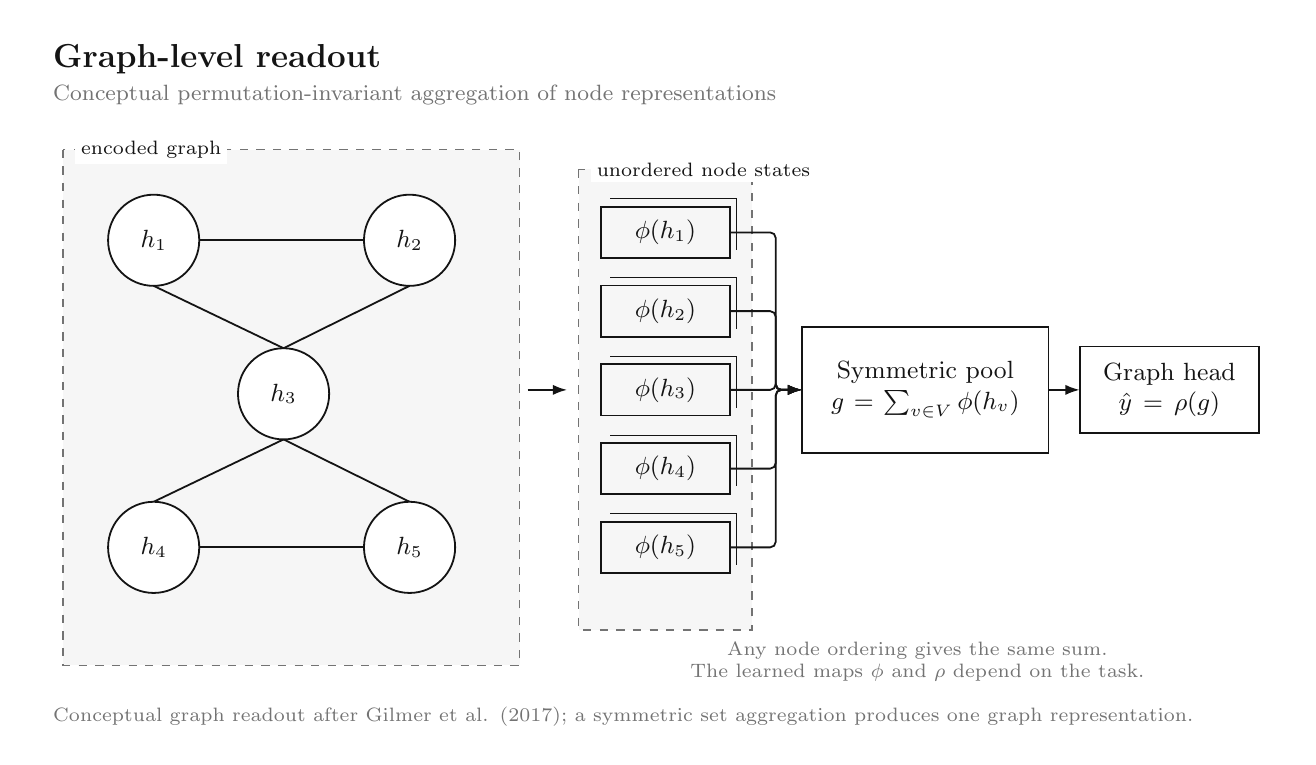
\begin{tikzpicture}[x=1cm,y=-1cm,font=\rmfamily,text=ink]

\path[use as bounding box] (0,0) rectangle (16,9);
\node[anchor=west,font=\large\bfseries] at (.2,.4) {Graph-level readout};
\node[anchor=west,font=\footnotesize,text=soft] at (.2,.85) {Conceptual permutation-invariant aggregation of node representations};
\begin{pgfonlayer}{background}
\draw[groupbox] (0.45,1.55) rectangle (6.25,8.1);
\node[anchor=west,font=\scriptsize,fill=white,inner sep=2pt] at (0.6,1.55) {encoded graph};
\draw[groupbox] (7.0,1.8) rectangle (9.2,7.6499999999999995);
\node[anchor=west,font=\scriptsize,fill=white,inner sep=2pt] at (7.15,1.8) {unordered node states};
\end{pgfonlayer}
\node[box,circle,minimum width=1.0cm,minimum height=1.0cm,text width=0.75cm] (v1) at (1.6,2.7) {$h_1$};
\node[box,circle,minimum width=1.0cm,minimum height=1.0cm,text width=0.75cm] (v2) at (4.85,2.7) {$h_2$};
\node[box,circle,minimum width=1.0cm,minimum height=1.0cm,text width=0.75cm] (v3) at (3.25,4.65) {$h_3$};
\node[box,circle,minimum width=1.0cm,minimum height=1.0cm,text width=0.75cm] (v4) at (1.6,6.6) {$h_4$};
\node[box,circle,minimum width=1.0cm,minimum height=1.0cm,text width=0.75cm] (v5) at (4.85,6.6) {$h_5$};
\node[box,fill=wash,minimum width=1.6cm,minimum height=0.65cm,text width=1.35cm] (h1) at (8.1,2.6) {$\phi(h_1)$};
\draw[ink,line width=.4pt] (7.3999999999999995,2.175) -- (9.0,2.175) -- (9.0,2.825);
\node[box,fill=wash,minimum width=1.6cm,minimum height=0.65cm,text width=1.35cm] (h2) at (8.1,3.6) {$\phi(h_2)$};
\draw[ink,line width=.4pt] (7.3999999999999995,3.175) -- (9.0,3.175) -- (9.0,3.825);
\node[box,fill=wash,minimum width=1.6cm,minimum height=0.65cm,text width=1.35cm] (h3) at (8.1,4.6) {$\phi(h_3)$};
\draw[ink,line width=.4pt] (7.3999999999999995,4.175) -- (9.0,4.175) -- (9.0,4.825);
\node[box,fill=wash,minimum width=1.6cm,minimum height=0.65cm,text width=1.35cm] (h4) at (8.1,5.6) {$\phi(h_4)$};
\draw[ink,line width=.4pt] (7.3999999999999995,5.175) -- (9.0,5.175) -- (9.0,5.825);
\node[box,fill=wash,minimum width=1.6cm,minimum height=0.65cm,text width=1.35cm] (h5) at (8.1,6.6) {$\phi(h_5)$};
\draw[ink,line width=.4pt] (7.3999999999999995,6.175) -- (9.0,6.175) -- (9.0,6.825);
\node[box,minimum width=3.1cm,minimum height=1.6cm,text width=2.85cm] (pool) at (11.4,4.6) {Symmetric pool\\$g=\sum_{v\in V}\phi(h_v)$};
\node[box,minimum width=2.25cm,minimum height=1.1cm,text width=2.0cm] (predict) at (14.5,4.6) {Graph head\\$\hat{y}=\rho(g)$};
\begin{pgfonlayer}{background}
\draw[flow,-] (v1.east) -- (v2.west);
\draw[flow,-] (v1.south) -- (v3.north);
\draw[flow,-] (v2.south) -- (v3.north);
\draw[flow,-] (v3.south) -- (v4.north);
\draw[flow,-] (v3.south) -- (v5.north);
\draw[flow,-] (v4.east) -- (v5.west);
\draw[flow] (h1.east) -- (9.5,2.6) -- (9.5,4.6) -- (pool.west);
\draw[flow] (h2.east) -- (9.5,3.6) -- (9.5,4.6) -- (pool.west);
\draw[flow] (h3.east) -- (9.5,4.6) -- (9.5,4.6) -- (pool.west);
\draw[flow] (h4.east) -- (9.5,5.6) -- (9.5,4.6) -- (pool.west);
\draw[flow] (h5.east) -- (9.5,6.6) -- (9.5,4.6) -- (pool.west);
\draw[flow] (pool.east) -- (predict.west);
\end{pgfonlayer}
\draw[flow] (6.35,4.6) -- (6.85,4.6);
\node[annotation,text width=8.4cm] at (11.3,8.05) {Any node ordering gives the same sum.\\The learned maps $\phi$ and $\rho$ depend on the task.};
\node[anchor=west,align=left,font=\scriptsize,text=soft,text width=15.6cm] at (.2,8.75) {Conceptual graph readout after Gilmer et al. (2017); a symmetric set aggregation produces one graph representation.};
\end{tikzpicture}
\end{document}
